\chapter{Stand der Technik}
Zur genaueren Einordnung von Smartglasses und deren Klassifikation müssen zunächst einige Grundlegende Begriffe geklärt werden. Smartglasses werden in der Literatur verschiedenen Kategorien zugeordnet. So werden sie als Head-Mounted- Displays (HMD), des Wearable Computing als auch des Ubiquitous Computing zugeordnet \cite[S.~20]{}. HMD umfassen sowohl Virtual Reality (VR)- Brillen, als auch Augmented Reality (AR)- Brillen.

\section{Einordnung von Smartglasses}
\todo{Guter Name?}
\emph{Virtual Reality (VR)} ist eine völlige Ersetzung der wahrgenommenen Realität durch eine virtuelle Realität. Dabei wird dem Nutzer das Gefühl vermittelt, \enquote{Teil einer virtuellen Realität zu sein.} \cite[S.~22]{ThomasDirkMetzgerHelmutNiegemannHrsg2018}. Virtual Reality-Brillen ermöglichen es dem Nutzer im gegensatz zu Augmented Reality- Brillen komplett in eine Virtuelle Realität abzutauchen. Realisiert wird dies durch vollständig geschlossene Gehäuse und Linsen, die vor dem Bildschirm befestigt sind. Mittels der Linsen vor dem OLED-Display wird ein scharfes Sehen in einem sehr nahen Bereich ermöglicht. Bei VR-Brillen wird zwischen Full-Feature, Mobile und Low-Budget VR-Brillen unterschieden. Full-Feature Brillen wie die Oculus Rift sind mit einer für jedes Auge separaten Full-HD-Auflösung mit hoher Bildwiederholungsrate ausgestattet und bieten dank einer leicht versetzten Anordnung einen dreidimensionalen Effekt. Der Anwender verliert durch diese Brillen das Gefühl, auf einen Bildschirm zu schauen und hat das Gefühl in einer virtuellen Realität zu sein. Die Außenwelt wird vollkommen ausgeblendet. Bewegungen mit dem Kopf werden automatisch auf die virtuelle Welt eingestellt. Nutzer bekommen das Gefühl vollkommen Teil der virtuellen Welt zu sein \cite[S.~22ff]{ThomasDirkMetzgerHelmutNiegemannHrsg2018}. Mobile- und Low-Budget-VR-Brillen wie die Samsung Gear sind Produkte, die mithilfe eines aufgesetzten Smartphones eine Virtuelle Realität erstellen.
\begin{figure}[htbp]
    \centering
    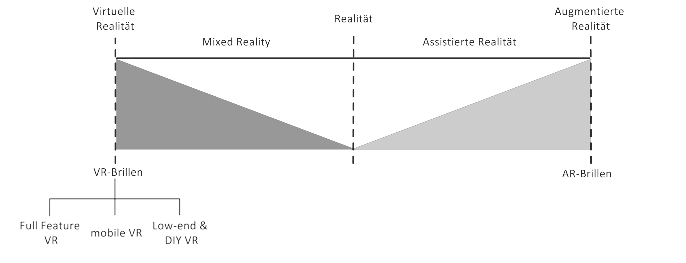
\includegraphics[width=1\textwidth]{data/bilder/VRvsAR.pdf}
    \caption{Einordnung von Smartglasses \cite{ThomasDirkMetzgerHelmutNiegemannHrsg2018}}
    \label{fig:mesh1}
\end{figure}
Unter \emph{Mixed Reality} wird eine Vermischung von realer Umgebung und virtueller Realität verstanden. Dabei wird eine Umgebung erstellt, in der reale und virtuelle Objekte kombiniert werden können. Darunter werden also Brillen verstanden, die komplett geschlossen sind und mittels einer Kamera Inhalte aus der realen Welt in die virtuelle Realität übertragen werden können.

\emph{Augmented Reality (AR)} ist im Gegensatz zu Virtual Reality das Einblenden von Informationen in das direkte Sichtfeld des Nutzers. Es wird also keine komplett virtuelle Realität erzeugt, sondern die reale Welt um digitale Inhalte ergänzt. Es gibt jedoch unterschiedliche Arten von Brillen, die Augmented Reality- Effekte erzeugen. Es wird differenziert zwischen Brillen, die \emph{echte} Augmented reality erzeugen und denen, die unterstützende Realität erzeugen. \emph{Echte} Augmented Reality wird durch Brillen wie die Microsoft Hololens erzeugt. Dabei werden kontextsensitive Informationen direkt ins Sichtfeld des Nutzers eingeblendet. Oberflächen-Erkennung ermöglicht eine Verschmelzung von realer Welt und digitalen Informationen. Die Hololens beispielsweise ist in der Lage, Dreidemensionale Hologramme im Sichtfeld des Nutzers anzuzeigen. Dies wird durch zwei transparente Displays ermöglicht.
Davon abzugrenzen ist eine assistierte Realität, die beispielsweise durch die Google Glass, die Realwear hmt1 oder die Vuzix M100/M300 erzeugt wird. Diese Brillen werden in der Literatur oft auch als Smartglasses bezeichnet \cite[S.~26]{ThomasDirkMetzgerHelmutNiegemannHrsg2018}. Bei diesen Brillen werden mittels eines sogenannten \emph{See Through Displays}, einem Prisma auf einem Auge, virtuelle Inhalte angezeigt, ohne Verlust der Realität mit sich zu ziehen. Steuern lassen sich AR-Brillen mittels optische Impulsgeber (Pick-by-Light) oder mobiler Hilfsmittel wie Headsets (Pick-by-Voice) \cite{INTRALOGISTIK2016}. Es ist also möglich per Gesten- oder Sprachsteuerung zu navigieren.
\todo{Mehr zu assistierte Realität}

\begin{comment}
Pick-by-vision Systeme, 
\end{comment}
%
% - - - - - - - - - - - - - - - - - - - - - - - - 
%
\section{Smartglasses im beruflichen Umfeld} \todo{Datenbrillen statt Smartglasses?}
% 3 Seiten
Die Logistikbranche is Deutschlands drittgrößte Branche \cite{Zobel2016}. In der Logistikbranche werden Datenbrillen in Form von Assistierten AR-Brillen (Smartglasses) eingesetzt. Smartglasses ermöglichen die Digtialisierung von Arbeitsprozessen. Sie ermöglichen die verbesserte Integration von Mitarbeitern in Unternehmensprozesse \cite{Zobel2016}. Smartglasses liefern Kontextabhängige Informationen beispielsweise via Barcodes bzw. QR-Codes. Angestellte der Logistikbranche der Transportlogistik werden in Echtzeit mit Informationen, wie beispielsweise Lieferaufträgen versorgt. Dabei müssen Arbeitsabläufe an sich nicht unterbrochen werden. In einer Use-Case-Studie \cite{Niemoller2017} wurden insgesamt 36 Einsatzmöglichkeiten für Smartglasses im Logistikdienstleistungssektor ermittelt. Die relevantesten Use-Cases werden im folgenden dargestellt:

Zum einen wurde das Themenfeld Kommunikation herausgearbeitet. Mittels Smartglasses ist das Anzeigen von Handlungsanweisungen sowie die Darstellung von Videoinformationen mittels Streaming oder offline-Videos möglich. Eine vereinfachte Kommunikation durch die Übersetzung von Texten ist ebenso möglich. Im Themenfeld Qualitätssicherung ist eine automatisierte Kontrolle mittels einer kamerabasierter Fehlererkennung sowie entsprechender Rückmeldung an den Nutzer möglich. Das Haupteinsatzfeld ist jedoch die Identifizierung anhand gespeicherter Merkmale wie Farbe, Größe und Geometrie oder auch durch die Identifizierung mittels Bar- und QR-Code \cite{Niemoller2017}. Identifizierung von Objekten ermöglicht die Anzeige von Zusatzinformationen. Im Themenfeld Sicherheit ist die Kontextabhängige Darstellung von Sicherheits- und Warnhinweisen möglich. 

Auf dem Fachkongress \emph{Smart Glasses Experience Days} \cite{Manokaran-Pathamathan2017} wurden weitere Einsatzfelder gezeigt. So können über die Datenbrille Montage- oder Reparaturanleitungen angezeigt werden. Es können zwecks Dokumentation Arbeitsschritte und Informationen des vorhergehenden Angestellten angezeigt werden. Per Remoteunterstützung können Angestellte Hilfe bei komplizierten Arbeitsschritten erhalten. Es können für Lagermitarbeiter Anweisungen angezeigt werden, wie und in welcher Reigenfolge Anweisungen befolgt werden sollen.

Neben der Logistikbranche werden Smartglasses auch in anderen Branchen eingesetzt. Der Studienbericht \emph{Smart Glasses in der Produktion} des Fraunhofer-Instituts für Produktionstechnologie IPT von 2016 \cite{Plutz} wurde der Einsatz von Smartglasses im beruflichen Umfeld der industriellen Produktion analysiert. So setzen 3,4\% der 237 befragten Unternehmen Unternehmen Smartglasses bereits ein. 15,1\% wollen diese in nächster Zeit einsetzen. Die häufigsten Anwendungsgebiete waren Mitarbeiterschulungen (27,3\%), Fernwartung/Videotelefonie (27,1\%), Echtzeitanzeige von Informationen (22,8\%) und industrielle Bildverarbeitung (17,5\%). Laut dem Bericht ist es möglich, nicht nur 
prozessrelevante Informationen zur Verfügung zu stellen, sondern Angestellte auch dazu zu befähigen, Informationen prozessintegriert zu erzeugen. Es sei zudem möglich, hochaufgelöste Zeiterfassung manueller Tätigkeiten zu realisieren und Prüfdaten nicht wie bislang handschriftlich digital zu erfassen, sondern dabei die Hände frei zu haben.

Laut einer Pressemitteilung des Logistikunternehmens DHL vom 2. August 2017 führt der Einsatz von Smartglasses zu einer 15-prozentigen Produktivitätssteigerung bei geringerer Fehlerquote in ihrer \cite{DeutschePostDHLGroup2017}. Mittels Sprachsteuerung lassen sich einzelne Kommissionieraufträge aufrufen und die nötigen Informationen auf dem Display anzeigen. So lassen sich Lagerort, Lagerplatz und die zu packende Anzahl der Ware anzeigen statt wie bisher auf papierbasierte Auftragsanweisungen zurückgreifen. Es kann freihändig gearbeitet werden.

Bosch setzt in seiner Logistiksparte ebenfalls Smartglasses ein. Für Bosch ist vor allem die Tatsache als für das Unternehmen von Vorteil, dass die Angestellten beim Scannen von Barcodes und QR-Codes die Hände freihaben \cite{Spinger2014}. 
%
% - - - - - - - - - - - - - - - - - - - - - - - - 
%
\section{Vergleich verschiedener Smartglasses}
% 2 Seiten
\todo{...}